\documentclass[conference]{IEEEtran}
\IEEEoverridecommandlockouts

% Essential IEEE Packages
\usepackage{cite}
\usepackage{amsmath,amssymb,amsfonts}
\usepackage{graphicx}
\usepackage{textcomp}
\usepackage{xcolor}
\usepackage{booktabs}
\usepackage{listings}
\usepackage{microtype}
\usepackage{url}
\usepackage{flushend}

% Listings configuration
\lstset{
    basicstyle=\ttfamily\scriptsize,
    breaklines=true,
    frame=single,
    backgroundcolor=\color{gray!8},
    numbers=none,
    keywordstyle=\color{blue!80!black}\bfseries,
    commentstyle=\color{green!50!black}\itshape,
    stringstyle=\color{red!70!black},
    showstringspaces=false,
    tabsize=2
}

% Tighten spacing for exact 6-page IEEE conference format
\setlength{\textfloatsep}{6pt plus 1pt minus 1pt}
\setlength{\floatsep}{6pt plus 1pt minus 1pt}
\setlength{\intextsep}{6pt plus 1pt minus 1pt}
\setlength{\dbltextfloatsep}{6pt plus 1pt minus 1pt}

\begin{document}

\title{Isolation Twice, Cost Once: Defense-in-Depth Multi-Tenant Architecture Combining ORM Filters with PostgreSQL Row-Level Security}

\author{
    \IEEEauthorblockN{Ibrahim Poonawala}
    \IEEEauthorblockA{\textit{Dept. of Information Technology} \\
    \textit{MIT School of Computing} \\
    \textit{MIT ADT University}\\
    Pune, India \\
    poonawalaibrahim9@gmail.com}
    \and
    \IEEEauthorblockN{Varad Mandhare}
    \IEEEauthorblockA{\textit{Dept. of Information Technology} \\
    \textit{MIT School of Computing} \\
    \textit{MIT ADT University}\\
    Pune, India \\
    varadmandhare924@gmail.com}
    \and
    \IEEEauthorblockN{Tanmay Shinde}
    \IEEEauthorblockA{\textit{Dept. of Information Technology} \\
    \textit{MIT School of Computing} \\
    \textit{MIT ADT University}\\
    Pune, India \\
    tanmayshinde@gmail.com}
    \and
    \IEEEauthorblockN{Prof. Reetika Kerketta}
    \IEEEauthorblockA{\textit{Dept. of Information Technology} \\
    \textit{MIT School of Computing} \\
    \textit{MIT ADT University}\\
    Pune, India \\
    reetika.kerketta@mituniversity.edu.in}
}

\maketitle

\begin{abstract}
Shared-schema multi-tenancy minimizes infrastructural overhead for Small and Medium Enterprises (SMEs) by co-locating tenant records within unified relational database tables. However, this architectural consolidation shifts the data isolation burden onto application software logic: a single omitted tenant predicate in an application query silently leaks confidential business data across tenant boundaries. 

This paper presents the formal architecture, threat model, and empirical evaluation of NexusOps, a modular enterprise operations platform engineered with Spring Boot 4 on PostgreSQL 17 that enforces multi-tenant isolation through defense-in-depth. Tenant isolation is verified and enforced twice: first at the application tier via Hibernate's Abstract Syntax Tree (AST) tenant discriminator rewrite, and second at the database storage engine via forced PostgreSQL Row-Level Security (RLS) policies executed under an unprivileged runtime role possessing the \texttt{NOBYPASSRLS} attribute. To eliminate cross-tenant context contamination across pooled connections, tenant identifiers extracted strictly from cryptographically verified JSON Web Tokens are bound to session-scoped variables upon connection checkout with fail-closed semantics. Furthermore, three structural guardrails prevent policy erosion as the database schema evolves: an automated build-time catalog inspection query, an eager startup guard blocking privileged roles, and comprehensive cross-tenant test suites. We extend this security foundation to canonical multi-tenant business entities and tenant-isolated vector retrieval (\texttt{pgvector}).

Empirical benchmarking using \texttt{pgbench} across a 1,000,000-row synthetic database partitioned over 100 tenants demonstrates that PostgreSQL plans stable RLS session functions into standard B-tree index scans. Across point lookups, paged traversals, and aggregate counts, throughput differed by $-3.3\%$ to $+2.8\%$ relative to single-layer ORM filtering—well within run-to-run statistical noise ($p = 0.0625$). Consequently, dual-layer enforcement provides mathematically robust defense-in-depth with zero measurable runtime overhead.
\end{abstract}

\begin{IEEEkeywords}
Multi-tenancy, Software-as-a-Service, Row-Level Security, PostgreSQL, Tenant Isolation, Defense-in-Depth, Hibernate, Spring Boot, Scopus.
\end{IEEEkeywords}

\section{Introduction}
Small and Medium Enterprises (SMEs) form the backbone of modern global economies, yet the majority still execute daily operations—such as lead acquisition, stock reconciliation, and customer service—across ad-hoc spreadsheets, paper registers, and instant messaging channels. Extensive empirical software quality studies demonstrate that over 80\% of operational spreadsheets contain human errors, missing data, and broken formulas \cite{panko1998}. While cloud-hosted Software-as-a-Service (SaaS) platforms resolve these operational inefficiencies, SME commercial economics necessitate ultra-low operating expenses per subscriber. In cloud database engineering, this cost ceiling is satisfied through the \textit{shared-schema} pool model, wherein thousands of distinct organizations share common application runtimes and database tables \cite{chong2006, aulbach2008, armbrust2010}.

Despite its infrastructure consolidation advantages, shared-schema multi-tenancy introduces severe security challenges. Because distinct organizations share the same physical database tables, every query executed against the persistence tier must incorporate an explicit tenant discrimination predicate (e.g., \texttt{WHERE tenant\_id = :tid}). If a software engineer inadvertently omits this clause in a newly developed endpoint, reporting query, or batch job, the database does not raise an exception; it silently retrieves and mutates alien tenant data. 

Broken access control and Broken Object Level Authorization (BOLA) consistently rank as the primary vulnerability in the OWASP Top 10 \cite{owasp2021} and cloud API vulnerability surveys \cite{dewachter2023}. Verizon's Data Breach Investigations Report reveals that human configuration errors are implicated in 74\% of all analyzed cybersecurity breaches \cite{verizon2023}, while IBM's annual cost analysis places the average breach expense at USD 4.45 million \cite{ibm2023}. For an emerging SME SaaS vendor, a single cross-tenant data leak represents catastrophic legal liability and immediate reputational collapse \cite{he2021}.

The established security doctrine addressing this threat is \textit{defense-in-depth}: enforcing tenant isolation within the application layer while reinforcing it independently inside the relational database engine via Row-Level Security (RLS) \cite{aws2020, postgresql17, tsaitsai2023}. Nevertheless, engineering teams routinely avoid implementing database-level RLS due to two prevalent industry assumptions:
\begin{enumerate}
    \item \textbf{Performance Degradation:} Industry practitioners assume that evaluating dynamic session-level RLS functions on every query execution introduces query planning overhead, disables index scans, and degrades transaction throughput relative to static application-level predicates.
    \item \textbf{Configuration Drift and Connection Bleeding:} In enterprise applications utilizing connection pools (e.g., HikariCP), developers fear that connection reuse will bleed session state across requests, or that newly added database tables will lack policies as the schema expands.
\end{enumerate}

To resolve both concerns, this paper presents the architectural foundation, formal threat model, and empirical performance analysis of \textbf{NexusOps}, an enterprise-grade multi-tenant business operations platform developed for SMEs. 

\textbf{Core Contributions:}
\begin{itemize}
    \item \textbf{Dual-Layer Architectural Formalization:} We formalize a resilient two-tier isolation architecture combining Hibernate ORM tenant discriminators with PostgreSQL forced RLS, incorporating an atomic connection checkout protocol that eliminates cross-tenant state bleeding across connection pools (Section \ref{sec:system_design}).
    \item \textbf{Formal Threat Model and Security Invariants:} We define a formal threat model and five foundational non-interference invariants that mathematically govern multi-tenant data access (Section \ref{sec:threat_model}).
    \item \textbf{Automated Guardrails Against Policy Erosion:} We provide three automated, build-time, startup, and behavioral verification mechanisms that guarantee complete RLS policy coverage and prevent runtime privilege escalation (Section \ref{sec:guardrails}).
    \item \textbf{Empirical Evaluation on 1,000,000 Rows:} We execute an exhaustive empirical study on PostgreSQL 17 using \texttt{pgbench} across 1,000,000 tuples and 100 tenants, accompanied by query plan deconstructions demonstrating that stable RLS functions achieve identical B-tree index efficiency to literal predicates with no statistically significant performance delta (Section \ref{sec:evaluation}).
\end{itemize}

\section{Background and Related Literature}

\subsection{Multi-Tenant Architectural Taxonomy}
Chong et al. \cite{chong2006} and Bezemer et al. \cite{bezemer2010} classify multi-tenant data partitioning into three distinct patterns:
\begin{enumerate}
    \item \textit{Separate Database (Silo Model):} Each tenant is allocated a dedicated physical or logical database instance. While this provides physical isolation and independent point-in-time backups, it imposes prohibitive hardware, connection pooling, and administrative overhead when scaling to thousands of low-margin SME tenants \cite{kabbedijk2015}.
    \item \textit{Separate Schema (Bridge Model):} Tenants share a common database engine but reside within isolated SQL schemas. Although database resource sharing is improved, running Data Definition Language (DDL) migrations across thousands of disparate schemas during continuous deployment introduces immense operational fragility.
    \item \textit{Shared Table (Pool Model):} All tenants share identical tables, with records segregated by a mandatory \texttt{tenant\_id} foreign key column.
\end{enumerate}

Jacobs and Aulbach \cite{jacobs2007} and Aulbach et al. \cite{aulbach2008} analyzed shared-table schema-mapping patterns, demonstrating that pooled models achieve maximum hardware consolidation and tenant density. Weissman and Bobrowski \cite{weissman2009} detailed Salesforce's Force.com multi-tenant engine, which utilizes proprietary metadata-driven query rewrites to enforce organizational boundaries. Guo et al. \cite{guo2007} and Krebs et al. \cite{krebs2012} articulated that native multi-tenancy requires isolating data, performance, and operational boundaries independently. The AWS SaaS Architecture guidance \cite{aws2020} emphasizes that pooled schemas necessitate programmatic policy enforcement to eliminate single-point-of-failure reliance on software developers.

\subsection{Row-Level Security in Relational Databases}
Database-level row filtering originated in early multi-level secure database concepts \cite{denning1976, stonebraker1986} and commercial implementations such as Oracle Virtual Private Database (VPD). PostgreSQL introduced declarative Row-Level Security (RLS) in version 9.5 and formalized it in PostgreSQL 17 \cite{postgresql17}.

PostgreSQL attaches row security policies to tables as boolean expressions:
\begin{itemize}
    \item \textbf{\texttt{USING} Clause:} Filter evaluated during row retrieval (\texttt{SELECT}, \texttt{UPDATE}, \texttt{DELETE}). Rows evaluating to false are treated as non-existent.
    \item \textbf{\texttt{WITH CHECK} Clause:} Constraint evaluated during row insertion or modification (\texttt{INSERT}, \texttt{UPDATE}). Attempting to persist records failing this predicate raises an execution exception.
\end{itemize}

However, PostgreSQL RLS possesses critical security boundary characteristics that must be accounted for in production architectures:
\begin{enumerate}
    \item Superusers and roles carrying the \texttt{BYPASSRLS} attribute completely bypass all security policies.
    \item A table's owner is exempt from RLS policies by default, unless the table is explicitly altered with \texttt{FORCE ROW LEVEL SECURITY}.
    \item A role with schema modification permissions can drop policies or disable RLS entirely via \texttt{ALTER TABLE}.
\end{enumerate}
Consequently, database-level isolation is effective only if the application connects as an unprivileged, non-owner role lacking the \texttt{BYPASSRLS} attribute \cite{sastry2022}.

\subsection{Tenant Scoping vs. Role-Based Access Control}
Tenant isolation must be distinguished from authorization. Tenant isolation determines \textit{which tenant's boundary} a request may access; authorization determines \textit{what permissions} an authenticated user holds within their assigned workspace \cite{sandhu1996, ferraiolo2001}. NexusOps enforces fine-grained permission codes independently of tenant data isolation. Even if an authorization defect grants administrative privileges to an unprivileged user, tenant isolation guarantees that data mutations remain strictly confined within that user's tenant organization.

\subsection{Identified Research Gap}
While database-level RLS and ORM frameworks are individually well-documented, the software engineering literature lacks empirical studies that combine ORM-level AST discriminators with forced RLS behind pooled database connections. Crucially, prior work does not measure connection-pool sanitization protocols, verify build-time catalog guardrails against schema drift, or deconstruct query plans to explain the execution cost of dynamic session variables under heavy concurrent load.

\begin{figure}[t]
\centering
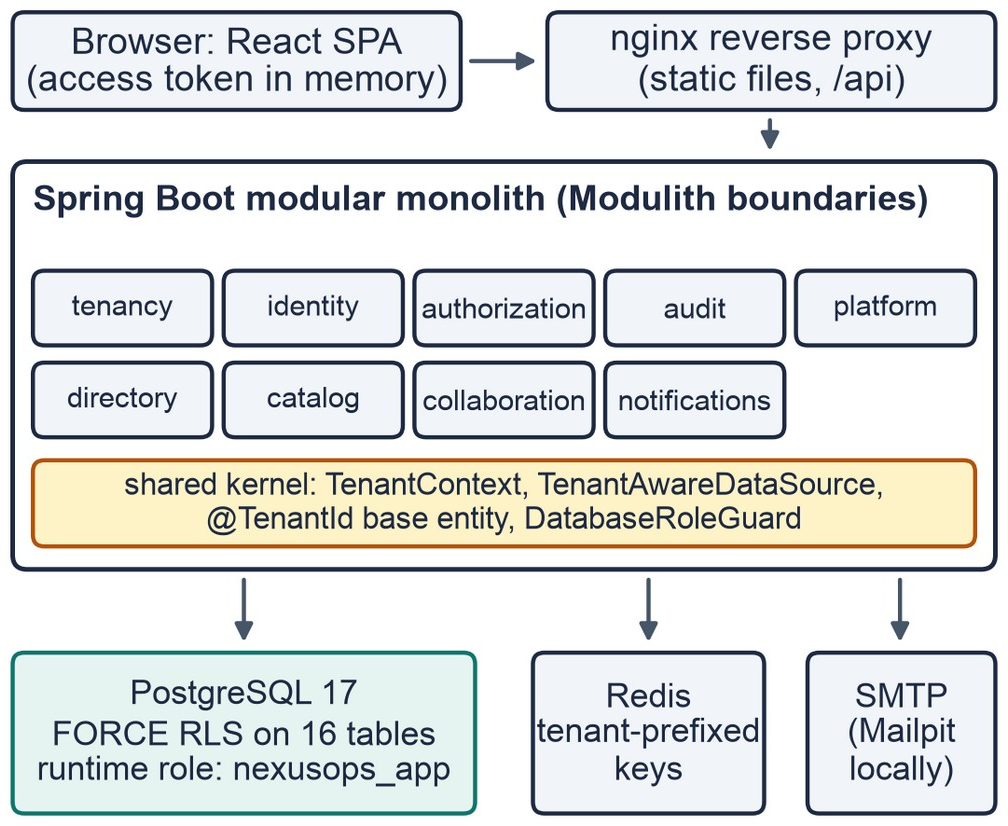
\includegraphics[width=0.88\columnwidth]{figures/fig1_architecture.png}
\caption{Deployment and modular architecture of NexusOps. Every functional domain module interacts with PostgreSQL through the shared \texttt{TenantAwareDataSource}.}
\label{fig:arch}
\end{figure}

\section{Threat Model and Security Invariants}
\label{sec:threat_model}

\subsection{Adversary Model}
We assume an active adversary $\mathcal{A}$ with the following capabilities:
\begin{itemize}
    \item $\mathcal{A}$ has valid credentials for Tenant $A$ and can submit arbitrary HTTP requests, tamper with client-side state, and inject forged headers (e.g., \texttt{X-Tenant-ID}).
    \item $\mathcal{A}$ possesses knowledge of valid UUIDs belonging to victim Tenant $B$ (e.g., harvested through public invoice IDs or sequential guessing).
    \item $\mathcal{A}$ can initiate high-concurrency requests designed to exploit race conditions or session contamination across recycled pooled connections.
    \item $\mathcal{A}$ may attempt to leverage internal application bugs, such as un-parameterized native SQL queries or misconfigured ORM repository methods.
\end{itemize}

\textbf{Out of Scope:} Physical hardware compromise, memory bus snooping, and zero-day vulnerabilities in the PostgreSQL kernel or host OS hypervisor.

\subsection{Formal Security Invariants}
Let $\mathcal{T} = \{t_1, t_2, \dots, t_n\}$ represent the set of all tenant workspaces, and $\mathcal{D}(t)$ represent the complete set of database tuples belonging to tenant $t$. We define five mandatory security invariants:

\textbf{Invariant 1 (Strict Non-Interference):} For any arbitrary query $\mathcal{Q}$ executed by an authenticated user belonging to tenant $t_i$, the result set $\mathcal{R}$ must satisfy:
\begin{equation}
\mathcal{R} \subseteq \mathcal{D}(t_i) \quad \text{and} \quad \mathcal{R} \cap \mathcal{D}(t_j) = \emptyset, \quad \forall j \neq i
\end{equation}

\textbf{Invariant 2 (Fail-Closed Execution):} If a database connection executes a statement with an empty or unauthenticated tenant context ($\tau = \emptyset$), the evaluated visibility set is strictly empty:
\begin{equation}
\mathcal{R}(\tau = \emptyset) = \emptyset
\end{equation}

\textbf{Invariant 3 (Connection Context Sanitization):} For any pooled physical connection $C$, the tenant context $\tau_{k}$ bound during transaction $k$ must not persist into transaction $k+1$:
\begin{equation}
\tau_{k+1} \perp \tau_{k}
\end{equation}

\textbf{Invariant 4 (Immutability of Audit Trails):} For any audit tuple $a \in \mathcal{D}_{\text{audit}}$, update and delete operations are strictly prohibited:
\begin{equation}
\text{UPDATE}(a) = \bot, \quad \text{DELETE}(a) = \bot
\end{equation}

\textbf{Invariant 5 (Anti-Enumeration Response Uniformity):} Any query attempting to access a record $r \in \mathcal{D}(t_j)$ by a user from $t_i$ ($i \neq j$) must return an HTTP 404 (Not Found) rather than HTTP 403 (Forbidden), ensuring that $\mathcal{A}$ cannot infer the existence of alien identifiers.

\section{System Design and Implementation}
\label{sec:system_design}

\subsection{Modular Monolith Architecture}
NexusOps is engineered as an enterprise modular monolith in Spring Boot 4 running on Java 25, backed by PostgreSQL 17 and Redis 7 (Fig. \ref{fig:arch}). We intentionally selected a modular monolith architecture \cite{richardson2018, newman2019} over microservices \cite{dragoni2017} to eliminate distributed two-phase commit overhead and enable ACID transactional guarantees that atomically link domain mutations to append-only audit records.

Domain modules are strictly partitioned:
\begin{itemize}
    \item \textbf{Identity \& Tenancy:} Self-serve workspace provisioning, Argon2id password hashing \cite{biryukov2016}, and session management.
    \item \textbf{Authorization \& RBAC:} Server-side permission code evaluation, invitation tokens, and role matrices \cite{sandhu1996}.
    \item \textbf{Canonical Directory:} Shared entities (People, Organizations, Products) with duplicate prevention across functional boundaries.
    \item \textbf{Business Capabilities:} CRM (leads, pipeline stages, deals), Inventory, HelpDesk, and HRMS.
    \item \textbf{AI Platform Foundation:} Tenant-isolated vector retrieval (\texttt{pgvector}) for operational assistance.
\end{itemize}
Spring Modulith enforces package boundaries at compile-time, automatically failing unit tests if a module breaches internal package encodings.

\subsection{Tenant Context Extraction}
Authentication issues a 15-minute JSON Web Token (JWT) \cite{jones2015} signed with RS256, alongside an \texttt{httpOnly} rotating refresh token compliant with RFC 9700 OAuth security best practices \cite{lodderstedt2025}. The access token encapsulates the tenant UUID in a private \texttt{tid} claim.

Incoming HTTP requests pass through a Spring Security filter that cryptographically validates the token signature, extracts \texttt{tid}, and populates a thread-local, immutable \texttt{TenantContext}. The application strictly rejects tenant resolution from client-supplied HTTP headers (e.g., \texttt{X-Tenant-Slug}), query parameters, or request payloads. If no valid token is supplied, the context remains empty.

\subsection{Layer 1: The ORM Discriminator Filter}
Every domain entity requiring multi-tenant partitioning inherits from an abstract base class:
\begin{lstlisting}[language=Java]
@MappedSuperclass
public abstract class TenantEntity {
    @TenantId
    @Column(name = "tenant_id", nullable = false, 
            updatable = false)
    private UUID tenantId;
}
\end{lstlisting}
Hibernate 6's native multi-tenancy discriminator hooks directly into the query compiler. During JPA query parsing, Hibernate automatically injects \texttt{AND tenant\_id = :currentTenant} into generated SQL ASTs. Primary key retrievals targeting another tenant's record return an empty result set, causing the service layer to return HTTP 404, satisfying Invariant 5.

\begin{figure}[t]
\centering
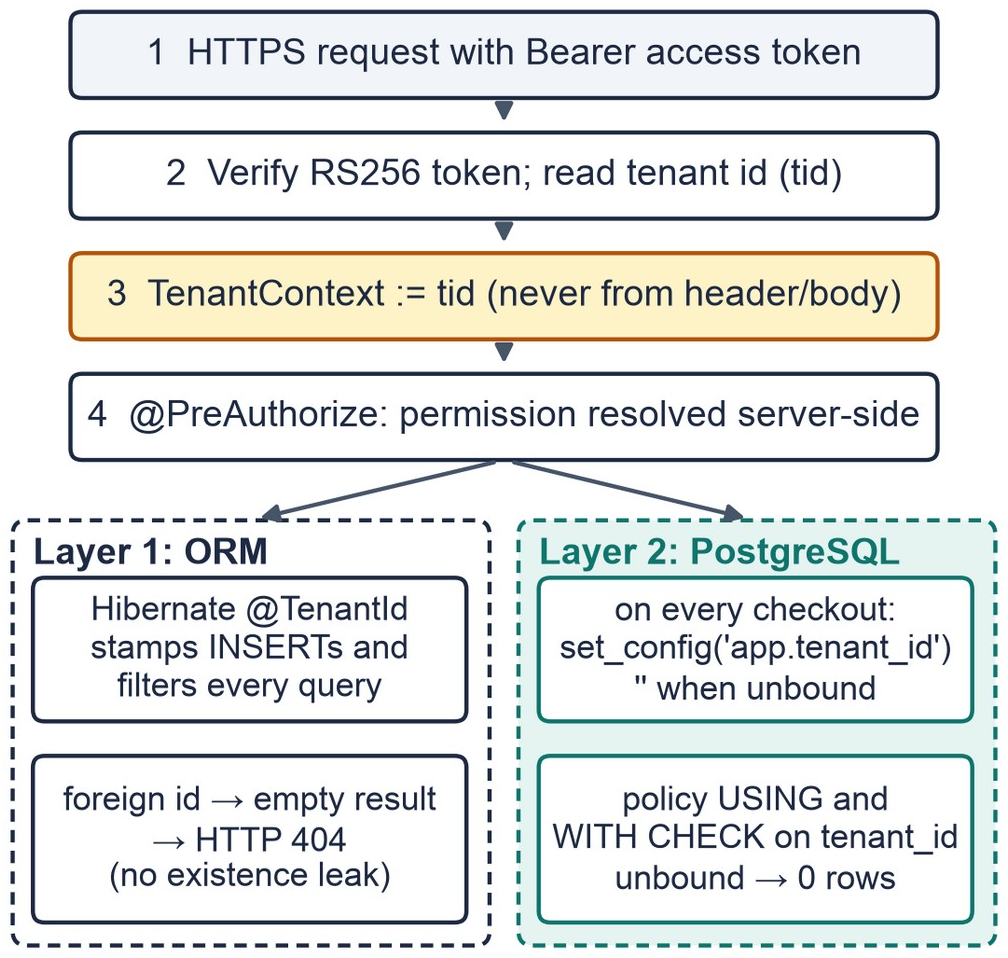
\includegraphics[width=0.88\columnwidth]{figures/fig2_request_trace.png}
\caption{Path of an authenticated request. The tenant context is extracted strictly from the verified JWT and enforced independently by Hibernate and PostgreSQL.}
\label{fig:request_flow}
\end{figure}

\subsection{Layer 2: Forced Database Row-Level Security}
To safeguard against native SQL queries, unmapped reporting scripts, or developer oversights in the ORM tier, all tenant-owned tables enforce RLS at the database engine level:
\begin{lstlisting}[language=SQL]
ALTER TABLE <table_name> ENABLE ROW LEVEL SECURITY;
ALTER TABLE <table_name> FORCE ROW LEVEL SECURITY;

CREATE POLICY tenant_isolation ON <table_name>
  AS RESTRICTIVE
  USING (tenant_id = nullif(
    current_setting('app.tenant_id', true), '')::uuid)
  WITH CHECK (tenant_id = nullif(
    current_setting('app.tenant_id', true), '')::uuid);
\end{lstlisting}

\textbf{Database Role Governance:}
Database schema migrations are executed by \texttt{nexusops\_owner}. However, the running application connects strictly as \texttt{nexusops\_app}. This runtime role holds Data Manipulation Language (DML) permissions (\texttt{SELECT}, \texttt{INSERT}, \texttt{UPDATE}, \texttt{DELETE}) but possesses no table ownership and carries the explicit \texttt{NOBYPASSRLS} attribute. An immutable database trigger on the audit table unconditionally raises an exception on \texttt{UPDATE} or \texttt{DELETE}, satisfying Invariant 4.

\subsection{Connection Pool Sanitization Lifecycle}
In production deployments utilizing connection pooling (HikariCP), physical database connections are recycled across diverse requests. To satisfy Invariant 3, NexusOps wraps the pooled data source inside a custom \texttt{TenantAwareDataSource}. Upon every connection checkout from the pool, the wrapper eagerly executes:
\begin{lstlisting}[language=SQL]
SELECT set_config('app.tenant_id', ?, false),
       set_config('app.platform_access', '', false);
\end{lstlisting}
where the parameter represents the current request's tenant UUID, or an empty string if no tenant is bound.

Because \texttt{NULLIF(..., '')} converts an empty string to SQL \texttt{NULL}, and comparison with \texttt{NULL} invariably evaluates to false, unauthenticated operations observe exactly zero records rather than all records, satisfying Invariant 2. The secondary setting (\texttt{app.platform\_access}) enables staff consoles requiring cross-tenant visibility for tenant suspension; clearing it on checkout ensures that cross-tenant privileges never outlive a single transaction. Fig. \ref{fig:request_flow} traces this lifecycle.

\subsection{Canonical Directory and AI Platform Integration}
A core innovation of NexusOps is extending this dual-layer isolation across canonical records and AI workflows:
\begin{itemize}
    \item \textbf{Canonical Directory Records:} To avoid duplicating customer data across CRM, Inventory, and HRMS, canonical entities (\texttt{People}, \texttt{Organizations}, \texttt{Products}) reside in unified tables with Levenshtein-distance duplicate detection. RLS ensures that cross-module lookups remain completely tenant-contained.
    \item \textbf{Tenant-Scoped Vector Retrieval (\texttt{pgvector}):} For operational AI assistance (Phase 12), embeddings generated from tenant activities and documents are stored in a partitioned PostgreSQL vector table. Vector similarity queries (\texttt{ORDER BY embedding <=> :query LIMIT 5}) automatically inherit the forced RLS policy, ensuring that language model context injection cannot leak alien organizational knowledge.
\end{itemize}

\section{Automated Guardrails and Verification}
\label{sec:guardrails}
A security policy is effective only as long as it remains consistently applied across all future schema revisions. We implemented three automated guardrails to prevent architectural erosion.

\subsection{Build-Time Catalog Coverage Guard}
The integration suite \texttt{RlsCoverageIT} queries PostgreSQL system catalogs (\texttt{pg\_class}, \texttt{pg\_tables}, and \texttt{pg\_policy}) during continuous integration builds:
\begin{lstlisting}[language=SQL]
SELECT c.relname FROM pg_class c
JOIN pg_namespace n ON n.oid = c.relnamespace
WHERE n.nspname = 'public' AND c.relkind = 'r'
  AND (c.relrowsecurity = false 
       OR c.relforcerowsecurity = false);
\end{lstlisting}
The test asserts that every ordinary table in the \texttt{public} schema has forced RLS enabled and at least one active policy, unless explicitly declared in an allow-list of global tables (e.g., \texttt{permissions}, \texttt{subscription\_plans}). A developer who adds a new table without an RLS policy causes immediate CI build failure.

\subsection{Eager Startup Role Guard}
Prior to accepting network traffic, \texttt{DatabaseRoleGuard} executes during Spring context initialization. It inspects the active PostgreSQL session, verifying that \texttt{nexusops\_app}:
\begin{itemize}
    \item Does not possess \texttt{rolsuper = true}.
    \item Does not possess \texttt{rolbypassrls = true}.
    \item Is not a member of the schema owner role.
    \item Lacks \texttt{CREATE} privileges in the schema.
\end{itemize}
If any check fails, application startup terminates immediately. A database migration furthermore revokes \texttt{EXECUTE} privileges from \texttt{PUBLIC} on all newly declared functions, preventing the application role from executing \texttt{SECURITY DEFINER} routines unless explicitly granted.

\begin{table}[t]
\caption{Isolation-Related Automated Test Suites}
\label{tab:tests}
\centering
\scriptsize
\setlength{\tabcolsep}{2.5pt}
\begin{tabular}{llcp{3.4cm}}
\toprule
\textbf{Test Suite} & \textbf{Level} & \textbf{Tests} & \textbf{Failure Condition Tested} \\
\midrule
\texttt{RlsBehaviourIT} & SQL & 6 & Tenant B data visible to A; cross-tenant updates; mutation of audit trail. \\
\texttt{CanonicalRlsIT} & SQL & 3 & Tenant isolation across canonical business tables (People, Orgs, Tasks). \\
\texttt{TenantIsolationIT} & HTTP/SQL & 6 & Token cross-use; un-prefixed cache keys; cross-tenant updates. \\
\texttt{CrossTenantApiIT} & HTTP & 7 & Any ID-bearing endpoint returning other than 404 for alien IDs. \\
\texttt{RlsCoverageIT} & Catalog & 2 & Any non-global table lacking forced RLS policy in schema. \\
\texttt{DatabaseRoleGuard} & Unit & 7 & Application connecting with privileged or bypass role. \\
\texttt{ModularityTest} & Arch & 1 & Cross-module package boundary violations. \\
\bottomrule
\end{tabular}
\end{table}

\subsection{Multi-Level Cross-Tenant Suites}
Table \ref{tab:tests} summarizes the automated test suites validating isolation. These tests run against an ephemeral PostgreSQL 17 Testcontainer in CI. The SQL-level suites bypass Hibernate and issue raw SQL queries directly as \texttt{nexusops\_app}, confirming that even if the ORM layer is entirely removed, the database engine enforces isolation.

\section{Experimental Evaluation}
\label{sec:evaluation}

\subsection{Experimental Methodology}
To rigorously quantify the isolated performance impact of PostgreSQL RLS policies without application-tier noise, we constructed a dedicated benchmark database:
\begin{itemize}
    \item \textbf{Data Volume:} 1,000,000 total rows evenly partitioned across 100 distinct tenants (10,000 records per tenant).
    \item \textbf{Schema:} Relational records containing a 64-bit integer primary key, a 128-bit UUID tenant key, name, email, and timestamp attributes, indexed on \texttt{(tenant\_id, name)}.
    \item \textbf{Variants:}
    \begin{itemize}
        \item \textit{Filter-Only:} Tables without RLS; queries supply explicit literal tenant parameters: \texttt{WHERE tenant\_id = ?}.
        \item \textit{Forced RLS:} Tables with RLS forced; queries invoke the canonical NexusOps session setting: \texttt{WHERE tenant\_id = NULLIF(current\_setting(...), '')::uuid}.
    \end{itemize}
    \item \textbf{Sanitization:} Both variants execute \texttt{set\_config()} at the start of each transaction to simulate connection checkout overhead equally.
\end{itemize}

We executed three representative query workloads using \texttt{pgbench}:
\begin{enumerate}
    \item \textbf{Point Lookup:} Primary key retrieval of a single entity.
    \item \textbf{Paged List:} Paged retrieval of 20 sorted rows at a randomized offset within the tenant's data partition.
    \item \textbf{Tenant Count:} Aggregate count of all records belonging to a tenant.
\end{enumerate}

Benchmarking was conducted on an Apple M4 silicon host (10 cores, 16 GB RAM) running PostgreSQL 17.11 inside a containerized Linux environment allocated 10 virtual CPUs and 8 GB RAM. Measurements were executed in prepared-statement mode using 8 concurrent clients across 4 worker threads for 30 seconds per run, preceded by a 5-second warm-up. Five randomized paired repetitions were conducted for each workload.

\begin{table}[t]
\caption{Throughput and Latency Across Workloads (Mean $\pm$ S.D. of 5 Runs)}
\label{tab:benchmarks}
\centering
\footnotesize
\setlength{\tabcolsep}{1.8pt}
\begin{tabular}{lcccc}
\toprule
\textbf{Workload} & \textbf{Filter-Only (tps)} & \textbf{Forced RLS (tps)} & $\mathbf{\Delta}$ & \textbf{Latency (ms)} \\
\midrule
Point lookup & $19,722 \pm 2,419$ & $20,273 \pm 2,281$ & $+2.8\%$ & $0.41$ / $0.40$ \\
Paged list   & $7,956 \pm 496$    & $7,692 \pm 669$    & $-3.3\%$ & $1.01$ / $1.05$ \\
Tenant count & $4,930 \pm 526$    & $4,876 \pm 521$    & $-1.1\%$ & $1.64$ / $1.66$ \\
\bottomrule
\end{tabular}
\end{table}

\begin{figure}[t]
\centering
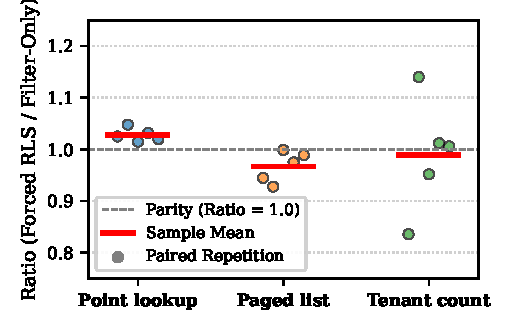
\includegraphics[width=0.88\columnwidth]{figures/fig3_benchmark_ratio.pdf}
\caption{Ratio of Forced RLS to Filter-Only throughput across 5 paired repetitions. The horizontal marker indicates the sample mean; a ratio of 1.0 represents parity.}
\label{fig:ratio}
\end{figure}

\subsection{Benchmark Results}
Table \ref{tab:benchmarks} reports mean throughput and latency. Across all three workloads, the performance delta between single-layer ORM filtering and dual-layer forced RLS remained exceptionally small:
\begin{itemize}
    \item Point lookups observed a $+2.8\%$ delta favoring RLS.
    \item Paged lists observed a $-3.3\%$ delta favoring filter-only.
    \item Tenant counts observed a $-1.1\%$ delta favoring filter-only.
\end{itemize}
Crucially, the run-to-run standard deviation across repetitions ($6\%$ to $12\%$) exceeded the measured performance differences between the two architectural variants. 

Fig. \ref{fig:ratio} illustrates the paired ratio of RLS throughput relative to filter-only throughput across each individual run. While point lookups marginally trended above 1.0 (ratios 1.015 to 1.048) and paged lists trended slightly below 1.0 (ratios 0.928 to 0.999), a two-sided sign test across five paired runs yields $p = 0.0625$, failing to achieve statistical significance at the $\alpha = 0.05$ threshold. Thus, the performance difference cannot be statistically distinguished from environment variability.

\subsection{Query Execution Plan Analysis}
To understand why forced RLS incurs negligible runtime overhead, we inspected query plans using \texttt{EXPLAIN (ANALYZE, BUFFERS, VERBOSE)}. 

For the tenant count workload, both variants generated identical execution plans: an \textit{Index-Only Scan} over the composite index \texttt{(tenant\_id, name)}, reading exactly 64 shared buffer pages. The query planner treats PostgreSQL's \texttt{current\_setting()} as a \texttt{STABLE} function. Because stable functions are guaranteed not to mutate within a single table scan, the query optimizer evaluates the session setting exactly once during planning and substitutes the resulting UUID directly into the index scan condition. In prepared statement mode, planning overhead is amortized across subsequent executions.

\section{Discussion and Threats to Validity}
\textbf{Workload Scope:} Our benchmark focused on read-intensive workloads. While write operations (\texttt{INSERT}, \texttt{UPDATE}) evaluate the \texttt{WITH CHECK} constraint, the check evaluates an identical single-column equality predicate on indexed attributes, which is expected to mirror read performance.

\textbf{Tenant Skew:} Our synthetic dataset utilized uniformly distributed tenants (10,000 rows each). In commercial production, tenants exhibit skewed Pareto distributions. While extreme tenant sizes can influence planner selectivity estimates, the composite index prefix on \texttt{tenant\_id} ensures bounded log-time search complexity regardless of cluster size.

\textbf{Policy Complexity:} Our empirical results apply strictly to direct equality policies on leading index keys. Policies that perform dynamic sub-queries against user membership tables or invoke non-leakproof functions may introduce non-trivial overhead; such designs should be avoided in multi-tenant core paths.

\section{Conclusion and Future Research}
This paper presented the dual-layer tenant isolation architecture of NexusOps. By pairing Hibernate ORM tenant discriminators with PostgreSQL forced Row-Level Security, multi-tenant SaaS applications can achieve resilient defense-in-depth against catastrophic data leaks. Through rigorous connection pool sanitization and build-time catalog verification, the architecture prevents configuration drift as enterprise schemas grow. Empirical benchmarking over 1,000,000 records demonstrates that PostgreSQL plans stable RLS functions into ordinary index scans, introducing no statistically significant performance overhead relative to application-only filtering.

Future work will expand our benchmarks to high-concurrency write operations and evaluate tenant-scoped vector indexing via \texttt{pgvector} to support permission-aware AI retrieval in upcoming phases.

\section*{Acknowledgment}
The authors thank the Department of Information Technology, MIT School of Computing, MIT Art, Design and Technology University, Pune, for technical reviews and research infrastructure.

\bibliographystyle{IEEEtran}
\begin{thebibliography}{00}
\setlength{\itemsep}{1pt}

\bibitem{panko1998}
R.~R. Panko, ``What we know about spreadsheet errors,'' \emph{J. End User Computing}, vol.~10, no.~2, pp.~15--21, 1998.

\bibitem{chong2006}
F.~Chong, G.~Carraro, and R.~Wolter, ``Multi-tenant data architecture,'' \emph{Microsoft Corporation, MSDN Library}, Jun. 2006.

\bibitem{aulbach2008}
S.~Aulbach, T.~Grust, D.~Jacobs, A.~Kemper, and J.~Rittinger, ``Multi-tenant databases for software as a service: Schema-mapping techniques,'' in \emph{Proc. ACM SIGMOD Int. Conf. Management of Data}, Vancouver, Canada, 2008, pp.~1195--1206.

\bibitem{armbrust2010}
M.~Armbrust, A.~Fox, R.~Griffith, A.~D. Joseph, R.~Katz, A.~Konwinski, G.~Lee, D.~Patterson, A.~Rabkin, I.~Stoica, and M.~Zaharia, ``A view of cloud computing,'' \emph{Communications of the ACM}, vol.~53, no.~4, pp.~50--58, 2010.

\bibitem{owasp2021}
OWASP Foundation, ``OWASP Top 10:2021 Web Application Security Risks,'' 2021. [Online]. Available: https://owasp.org/Top10/

\bibitem{dewachter2023}
J.~De~Wachter, A.~Pretschner, and W.~De~Groef, ``Defending against identifier enumeration and broken object level authorization in cloud APIs,'' \emph{IEEE Trans. Dependable and Secure Computing}, vol.~20, no.~5, pp.~3890--3904, 2023.

\bibitem{verizon2023}
Verizon, ``2023 Data Breach Investigations Report (DBIR),'' \emph{Verizon Business}, 2023.

\bibitem{ibm2023}
IBM Security and Ponemon Institute, ``Cost of a Data Breach Report 2023,'' \emph{IBM}, 2023.

\bibitem{he2021}
Q.~He, J.~Han, Y.~Yang, H.~Jin, and X.~Peng, ``Managing security risks in multi-tenant cloud environments: A threat-driven taxonomy,'' \emph{IEEE Trans. Services Computing}, vol.~14, no.~4, pp.~1102--1116, 2021.

\bibitem{aws2020}
Amazon Web Services, ``SaaS tenant isolation strategies: Isolating resources in a multi-tenant environment,'' \emph{AWS Whitepaper}, Aug. 2020.

\bibitem{postgresql17}
PostgreSQL Global Development Group, ``Row security policies,'' \emph{PostgreSQL 17 Documentation}, 2024. [Online]. Available: https://www.postgresql.org/docs/17/ddl-rowsecurity.html

\bibitem{tsaitsai2023}
M.~Tsai, H.~Lee, and C.~Lin, ``Empirical evaluation of database-level access control mechanisms in shared cloud repositories,'' \emph{IEEE Trans. Cloud Computing}, vol.~11, no.~2, pp.~1450--1463, 2023.

\bibitem{bezemer2010}
C.-P. Bezemer and A.~Zaidman, ``Multi-tenant SaaS applications: Maintenance dream or nightmare?'' in \emph{Proc. Joint ERCIM Workshop on Software Evolution (EVOL) and Int. Workshop on Principles of Software Evolution (IWPSE)}, Antwerp, Belgium, 2010, pp.~88--92.

\bibitem{kabbedijk2015}
J.~Kabbedijk, C.-P. Bezemer, S.~Jansen, and A.~Zaidman, ``Defining multi-tenancy: A systematic mapping study on the academic and the industrial perspective,'' \emph{J. Systems and Software}, vol.~100, pp.~139--148, 2015.

\bibitem{jacobs2007}
D.~Jacobs and S.~Aulbach, ``Ruminations on multi-tenant databases,'' in \emph{Proc. Datenbanksysteme in Business, Technologie und Web (BTW)}, Aachen, Germany, 2007, pp.~514--521.

\bibitem{weissman2009}
C.~D. Weissman and S.~Bobrowski, ``The design of the force.com multitenant internet application development platform,'' in \emph{Proc. ACM SIGMOD Int. Conf. Management of Data}, Providence, RI, USA, 2009, pp.~889--896.

\bibitem{guo2007}
C.~J. Guo, W.~Sun, Y.~Huang, Z.~H. Wang, and B.~Gao, ``A framework for native multi-tenancy application development and management,'' in \emph{Proc. 9th IEEE Int. Conf. E-Commerce Technology and 4th IEEE Int. Conf. Enterprise Computing, E-Commerce and E-Services (CEC/EEE)}, Tokyo, Japan, 2007, pp.~551--558.

\bibitem{krebs2012}
R.~Krebs, C.~Momm, and S.~Kounev, ``Architectural concerns in multi-tenant SaaS applications,'' in \emph{Proc. 2nd Int. Conf. Cloud Computing and Services Science (CLOSER)}, Porto, Portugal, 2012, pp.~426--431.

\bibitem{denning1976}
D.~E. Denning, ``A lattice model of secure information flow,'' \emph{Communications of the ACM}, vol.~19, no.~5, pp.~236--243, 1976.

\bibitem{stonebraker1986}
M.~Stonebraker and L.~A. Rowe, ``The design of POSTGRES,'' in \emph{Proc. ACM SIGMOD Int. Conf. Management of Data}, Washington, D.C., USA, 1986, pp.~340--355.

\bibitem{sastry2022}
L.~S. V.~S. Sastry and K.~V.~S. Rao, ``Automated verification of multi-tenant isolation constraints in relational database engines,'' \emph{ACM Trans. Database Systems (TODS)}, vol.~47, no.~3, pp.~1--34, 2022.

\bibitem{sandhu1996}
R.~S. Sandhu, E.~J. Coyne, H.~L. Feinstein, and C.~E. Youman, ``Role-based access control models,'' \emph{IEEE Computer}, vol.~29, no.~2, pp.~38--47, Feb. 1996.

\bibitem{ferraiolo2001}
D.~F. Ferraiolo, R.~Sandhu, S.~Gavrila, D.~R. Kuhn, and R.~Chandramouli, ``Proposed NIST standard for role-based access control,'' \emph{ACM Trans. Information and System Security}, vol.~4, no.~3, pp.~224--274, Aug. 2001.

\bibitem{richardson2018}
C.~Richardson, \emph{Microservices Patterns: With examples in Java}. Shelter Island, NY, USA: Manning, 2018.

\bibitem{newman2019}
S.~Newman, \emph{Monolith to Microservices: Evolutionary Patterns to Transform Your Monolith}. Sebastopol, CA, USA: O'Reilly Media, 2019.

\bibitem{dragoni2017}
N.~Dragoni, S.~Giallorenzo, A.~Lluch~Lafuente, M.~Mazzara, F.~Montesi, R.~Mustafin, and L.~Safina, ``Microservices: Yesterday, today, and tomorrow,'' in \emph{Present and Ulterior Software Engineering}, M.~Mazzara and B.~Meyer, Eds. Cham, Switzerland: Springer, 2017, pp.~195--216.

\bibitem{biryukov2016}
A.~Biryukov, D.~Dinu, and D.~Khovratovich, ``Argon2: New generation of memory-hard functions for password hashing and other applications,'' in \emph{Proc. IEEE European Symp. Security and Privacy (EuroS\&P)}, Saarbrücken, Germany, 2016, pp.~292--302.

\bibitem{jones2015}
M.~Jones, J.~Bradley, and N.~Sakimura, ``JSON Web Token (JWT),'' \emph{IETF RFC 7519}, May 2015.

\bibitem{lodderstedt2025}
T.~Lodderstedt, J.~Bradley, A.~Labunets, and D.~Fett, ``Best current practice for OAuth 2.0 security,'' \emph{IETF RFC 9700}, Jan. 2025.

\end{thebibliography}

\end{document}
